Another easy way to glance at recurrent event data is by event plots,
which can be created by applying the generic function \texttt{plot()} to
the \texttt{Recur} object when the \pkg{reReg} package is loaded.
Additionally, the \texttt{plotEvents()} function from the \pkg{reReg}
package allows users to stratify the event plots by discrete variables.
The following codes produces event plots with and without stratifying by
whether the patients receive chemotherapy.

\begin{Shaded}
\begin{Highlighting}[]
\NormalTok{df0 <-}\StringTok{ }\KeywordTok{subset}\NormalTok{(readmission, !(id %in%}\StringTok{ }\KeywordTok{c}\NormalTok{(}\DecValTok{60}\NormalTok{, }\DecValTok{109}\NormalTok{, }\DecValTok{280}\NormalTok{)))}
\NormalTok{obj <-}\StringTok{ }\KeywordTok{with}\NormalTok{(df0, }\KeywordTok{Recur}\NormalTok{(t.stop, id, event, death))}
\KeywordTok{plot}\NormalTok{(obj, }\DataTypeTok{legend =} \StringTok{"bottom"}\NormalTok{) ## no stratification}
\NormalTok{fn <-}\StringTok{ }\KeywordTok{Recur}\NormalTok{(t.stop, id, event, death) ~}\StringTok{ }\NormalTok{chemo}
\KeywordTok{plotEvents}\NormalTok{(fn, }\DataTypeTok{data =} \NormalTok{df0, }\DataTypeTok{legend =} \StringTok{"bottom"}\NormalTok{) ## by chemo}
\end{Highlighting}
\end{Shaded}

\vspace*{-.3cm}\begin{figure}[H]
\centering
\begin{subfigure}[t]{1.8in}
\centering
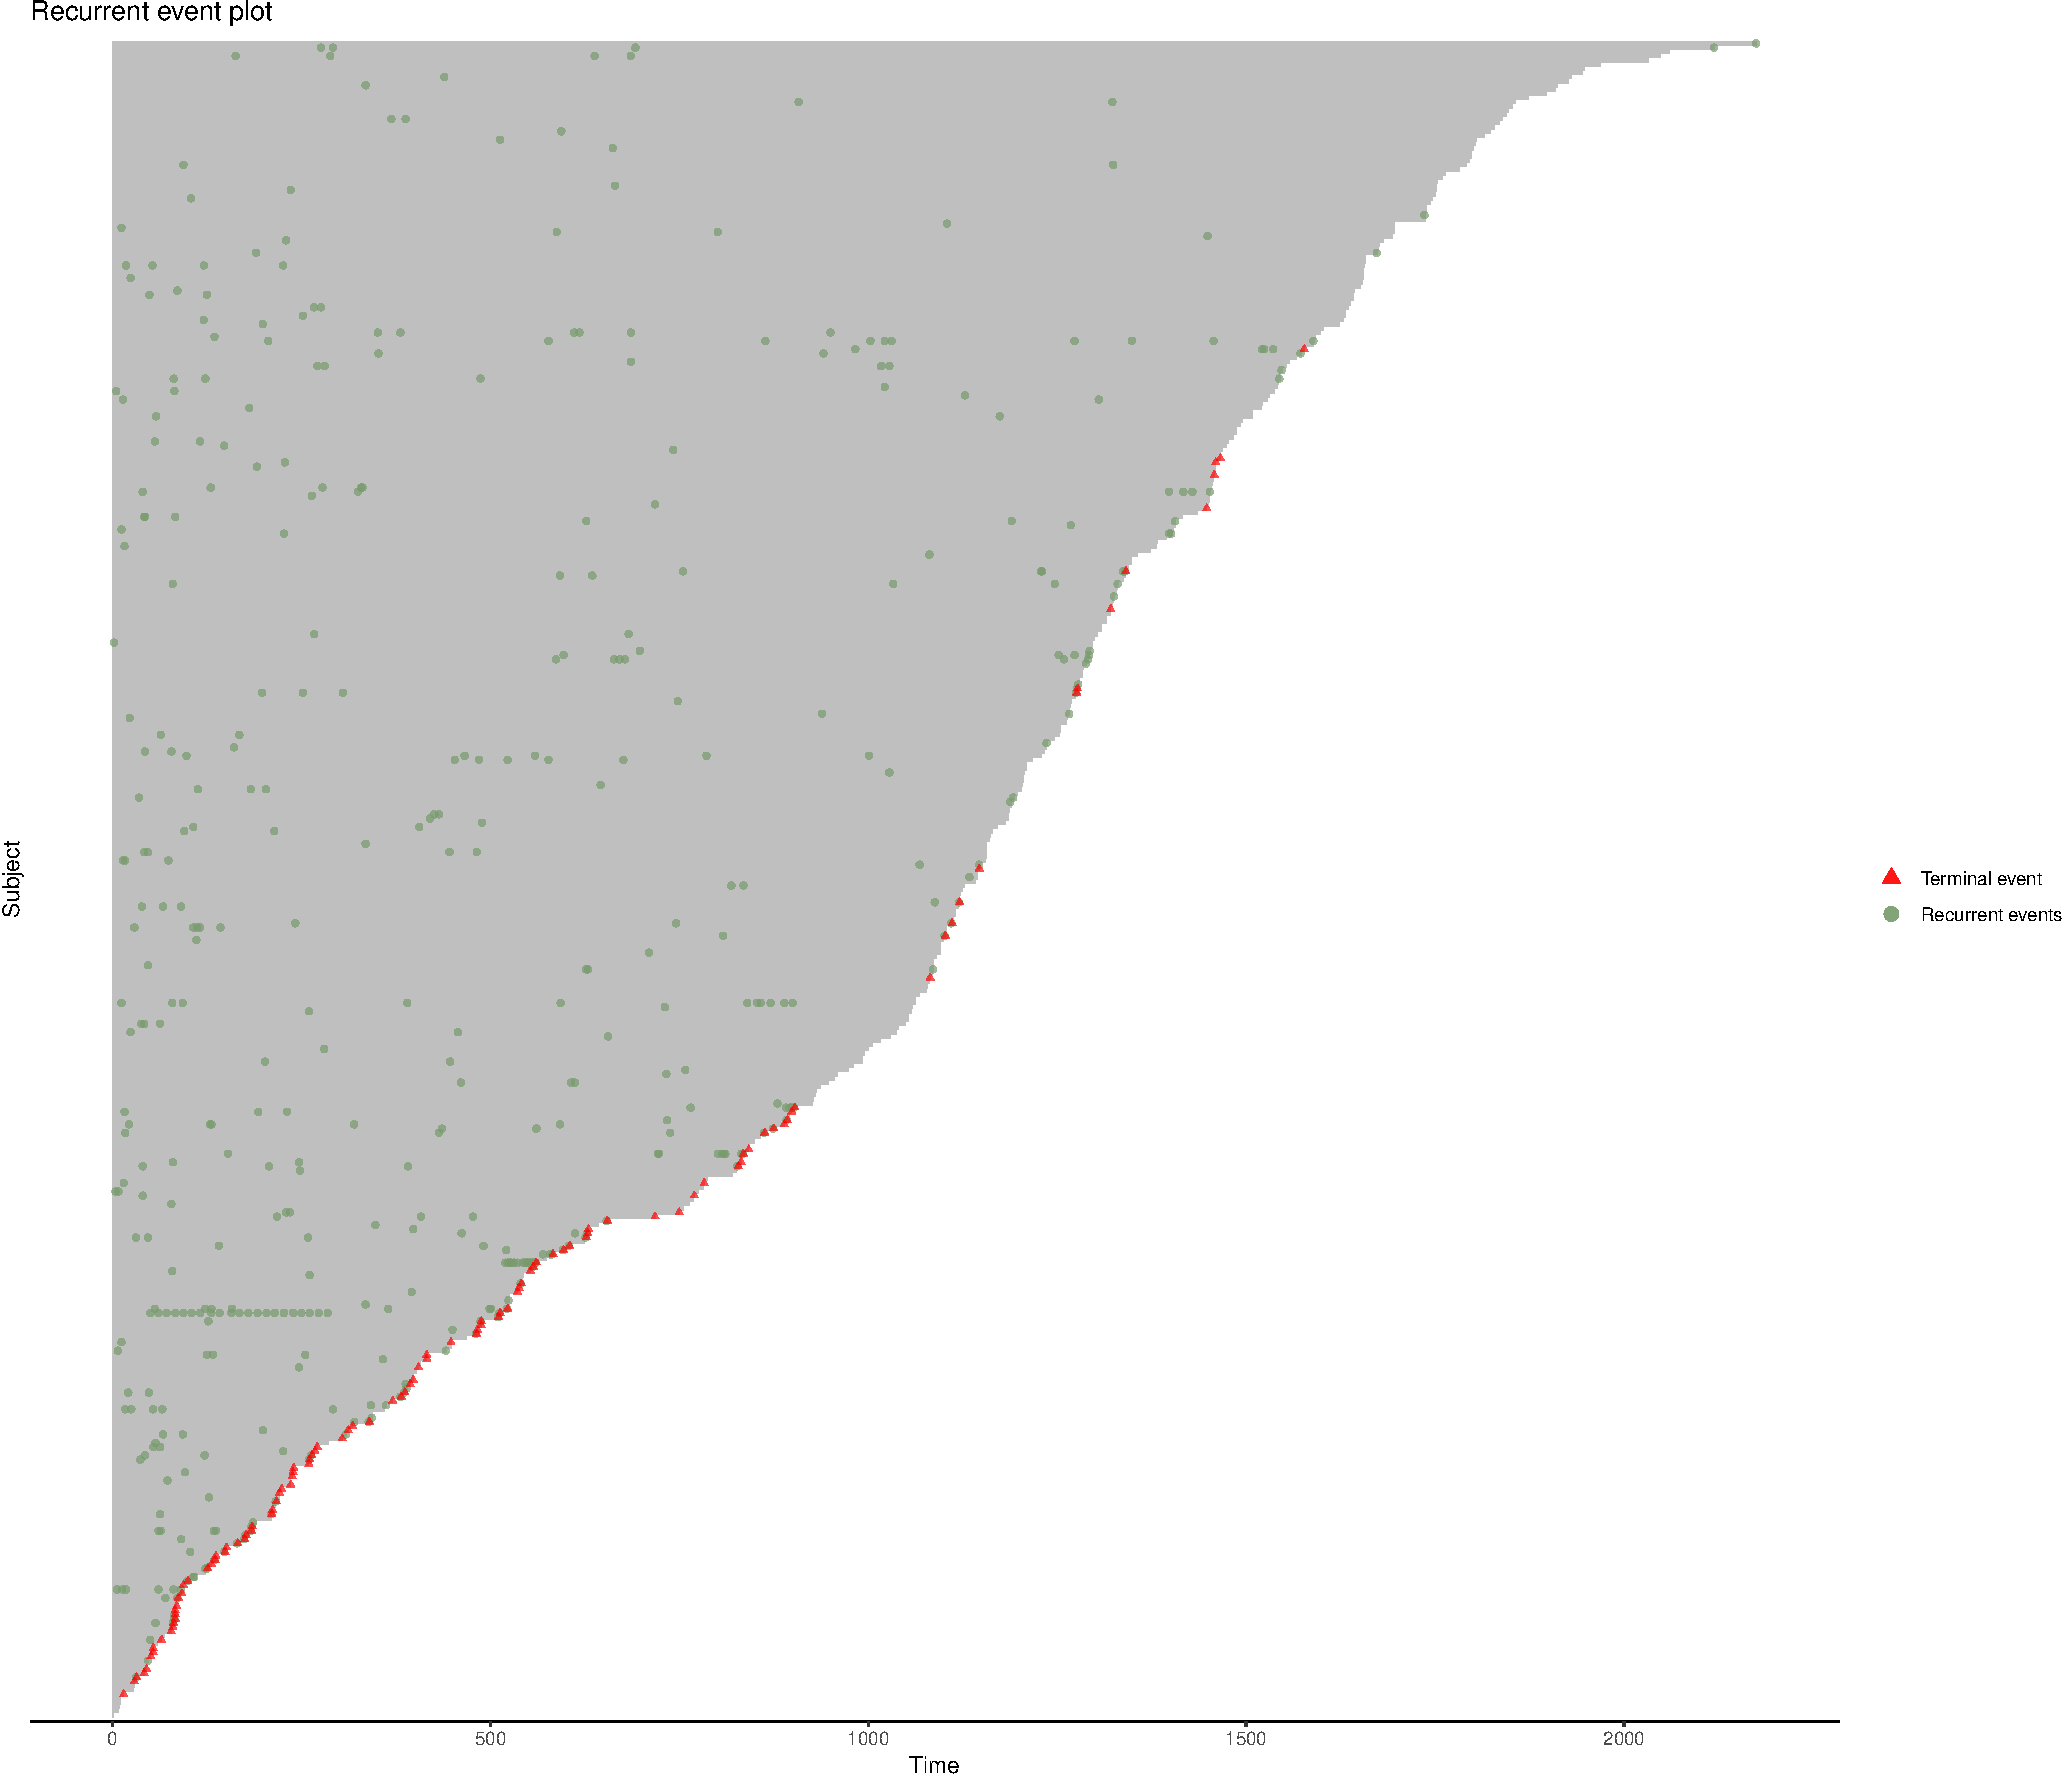
\includegraphics[scale = .125]{images/ep-1}
\caption{No stratification}\label{fig:1a}
\end{subfigure}
\quad
\begin{subfigure}[t]{1.8in}
\centering
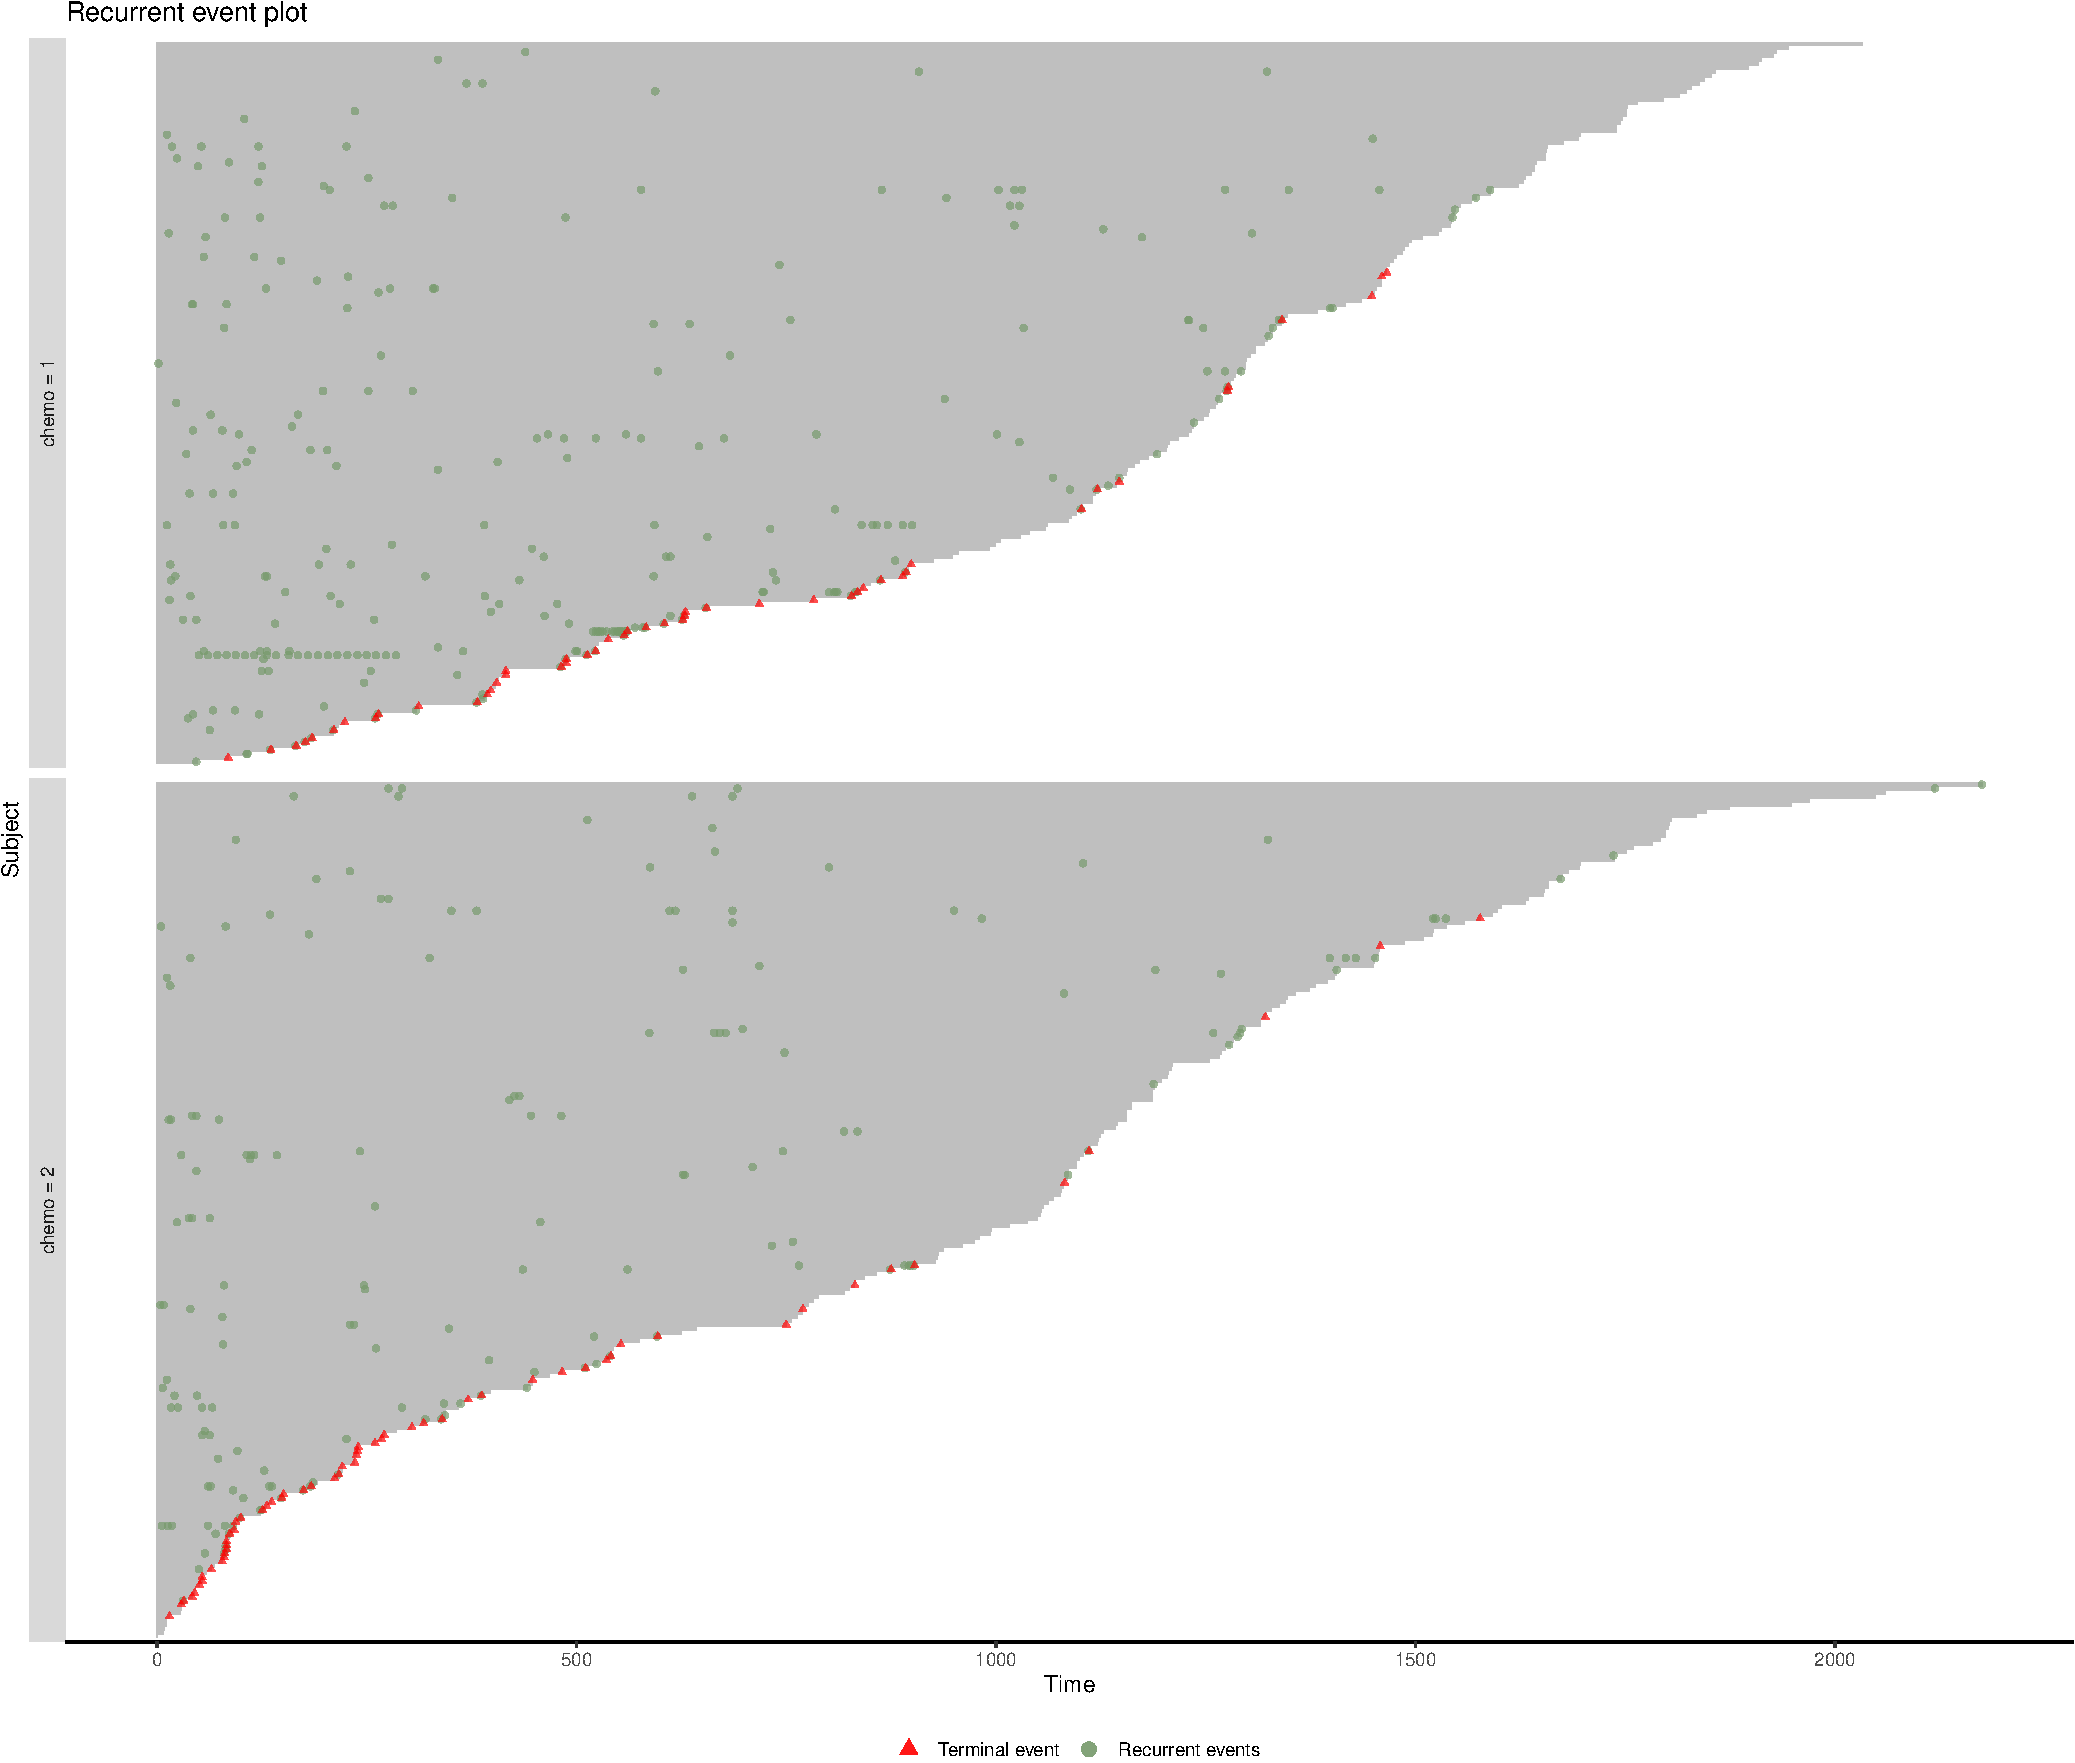
\includegraphics[scale = .125]{images/ep-2}
\caption{Stratified by \texttt{chemo}}\label{fig:1b}
\end{subfigure}
\caption{Event plots}\label{fig:1}
\end{figure}
